\chapter{Megvalósítás}

\section{Technológiák}

A felhasznált technológiákat a projekt fókuszai alapján választottuk ki. 
A választásunk a C++-ra esett, annak példátlan sebességéből, és a memória kezelését illető sajátosságaiból. Beépített könyvtára képmanipulációra viszont nincsen, ehhez az \href{https://en.wikipedia.org/wiki/OpenCV}{OpenCV} könyvtárat választottuk, annak nyílt forráskódja és optimalizáltsága miatt.
A felhasználói felülethez egy szintén platformfüggetlen megoldást szerettünk volna, ezért a \href{https://en.wikipedia.org/wiki/Qt_(software)}{Qt} melett döntöttünk. 

\section{Fejlesztést segítő eszközök}

A kooperációt a GitHub terveztük lebonyolítani, és tervben voltak GitHub actionök automatikus ellenőrzésekre is. A program buildeléséhez több másik próbálkozás után a \href{https://en.wikipedia.org/wiki/Meson_(software)}{Meson}t választottuk. A tervezéshez szükséges diagramokhoz \href{https://en.wikipedia.org/wiki/PlantUML}{PlantUML}-t használtam, fejlesztői környezetnek pedig a \href{https://en.wikipedia.org/wiki/Visual_Studio_Code}{Visual Studio Code}-ot

\section{Fejlesztés és nehézségek}

\subsection{Buildelés}

A legelső nehézség már fejlesztés legelején szembe jött velünk: a buildelés. Egyikünknek sem volt sok tapasztalata a build rendszerekkel, ezért erre sok időnk elment. Külön kihívás volt, külső könyvtárakat is linkelnünk kellett, amiknek a további konfigurációja messze nem volt triviális. Eleinte a \href{https://en.wikipedia.org/wiki/CMake}{CMake}-kel és a \href{https://en.wikipedia.org/wiki/Vcpkg}{vcpkg}-vel próbálkoztunk, de nem sikerült működésre bírnunk. Egy barátom, Bánáti Benedek javaslatára kezdtük el használni a Mesont, ami sokkal barátságosabbnak bizonyult. A Meson használata során is ütköztem további problémákba, mert a Qt header fájlokat a fordítás előtt még fel kell dolgozni, és erre csak CMake-es példákat találtam.

Indokalatlanul sok időnk ment rá, és Windowson azóta sem tudunk buildelni\footnote{nem lehetetlen, csak Windowson egy nagyságrenddel macerásabb előkészíteni a buildelési környezetet}, de ez sajnos a C++ velejárója.

\subsection{Modell és generálás}

A modell implementálása a tervek alapján gördülékenyen ment, és a régi módszerrel való generálás prototípusa is hamar elkészült. A prototípus sebességével elégedett voltam, nagyságrendekkel gyorsabb volt, mint ugyan ez Photoshopban. A strip tiling algoritmust megegyezés szerint Levi készítette volna, ennek az implementálására viszont nem került még sor, kollégám sűrű negyedik félévéből adódóan.

\subsection{A Qt és a felhasználói felület}

Ehhez a projekthez használtam először Qt-ot, ezért eleinte nagyon lassan haladt a felület fejlesztése. A Qt Quick használata mellett döntöttem, melynek segítségével egy deklaratív UI leíró nyelven (\href{https://en.wikipedia.org/wiki/QML}{QML}) lehet elkészíteni a felhasználó felületet. Néhány dologban hasonlít más UI leíró nyelvekre, nem kellett nulláról kezdenem, de azért még így is akadtak nehézségek bőven. Legfőképp a view és a modell összeköttetése, amivel hamar szembe találtam magam. Hogy egy osztályt elérnjünk QML-ből, ahhoz az osztályunknak nem elég a Qt osztályokból származnija, hanem még különféle makrókkal el kell lássuk a tagváltozóinkat, a függvényeinket, és még az osztályainkait is. Ezen osztályok header fájljait fordítás előtt fel kell dolgoznunk a Qt MOC\footnote{Meta-Object Compiler}-ével, hogy az osztályaink elérhetőek legyenek QML-ből, és hogy ezekről futásidejű típusinformációink is legyenek. 

Túlságosan nem mennék részletekbe a UI-t illetően, csupán pár érdekesebb részt emelnék ki. A lista, amin a bemenetek láthatóak lusta, azaz a nem látható elemeket és a hozzá tartozó állapotot és objektumokat a rendszer felszabadítja. Ezt az implementáció során figyelembe is vettem, és egy indirekcióval oldottam meg, arra viszont nem figyeltem, hogy a filterek modelljével való összeköttetés UI szinten valósult meg, és ez az összeköttetés csak addig van jelen, amíg az elem látható. Erre sajnos csak az éles tesztnél találtam rá, mert itt teszteltem először háromnál több képpel a programot. A hiba azóta javítva lett.

Egy másik érdekesség talán az előbeállítások betöltésének folyamata. A program JSON fájlokból olvas be, ezek létezését először az adott mappában felderíti, majd rögzíti a név és elérési út párokat. Betöltéskor a JSON-ben jelenlévő értékek felülírják az eddigi beállításainkat, a nem szereplő beállítások pedig nem lesznek hatással. A beállítások a már említett módon elkülönülnek (papír, dokumentum, nyomtató), de tovább tudnak propagálni más részekre. Így lehetséges például az, hogy a nagyplakát papírbeállítás hatással van a tekercs szélességére, vagy a matrica beállítás a képpontsűrűségre. 

\begin{figure}
    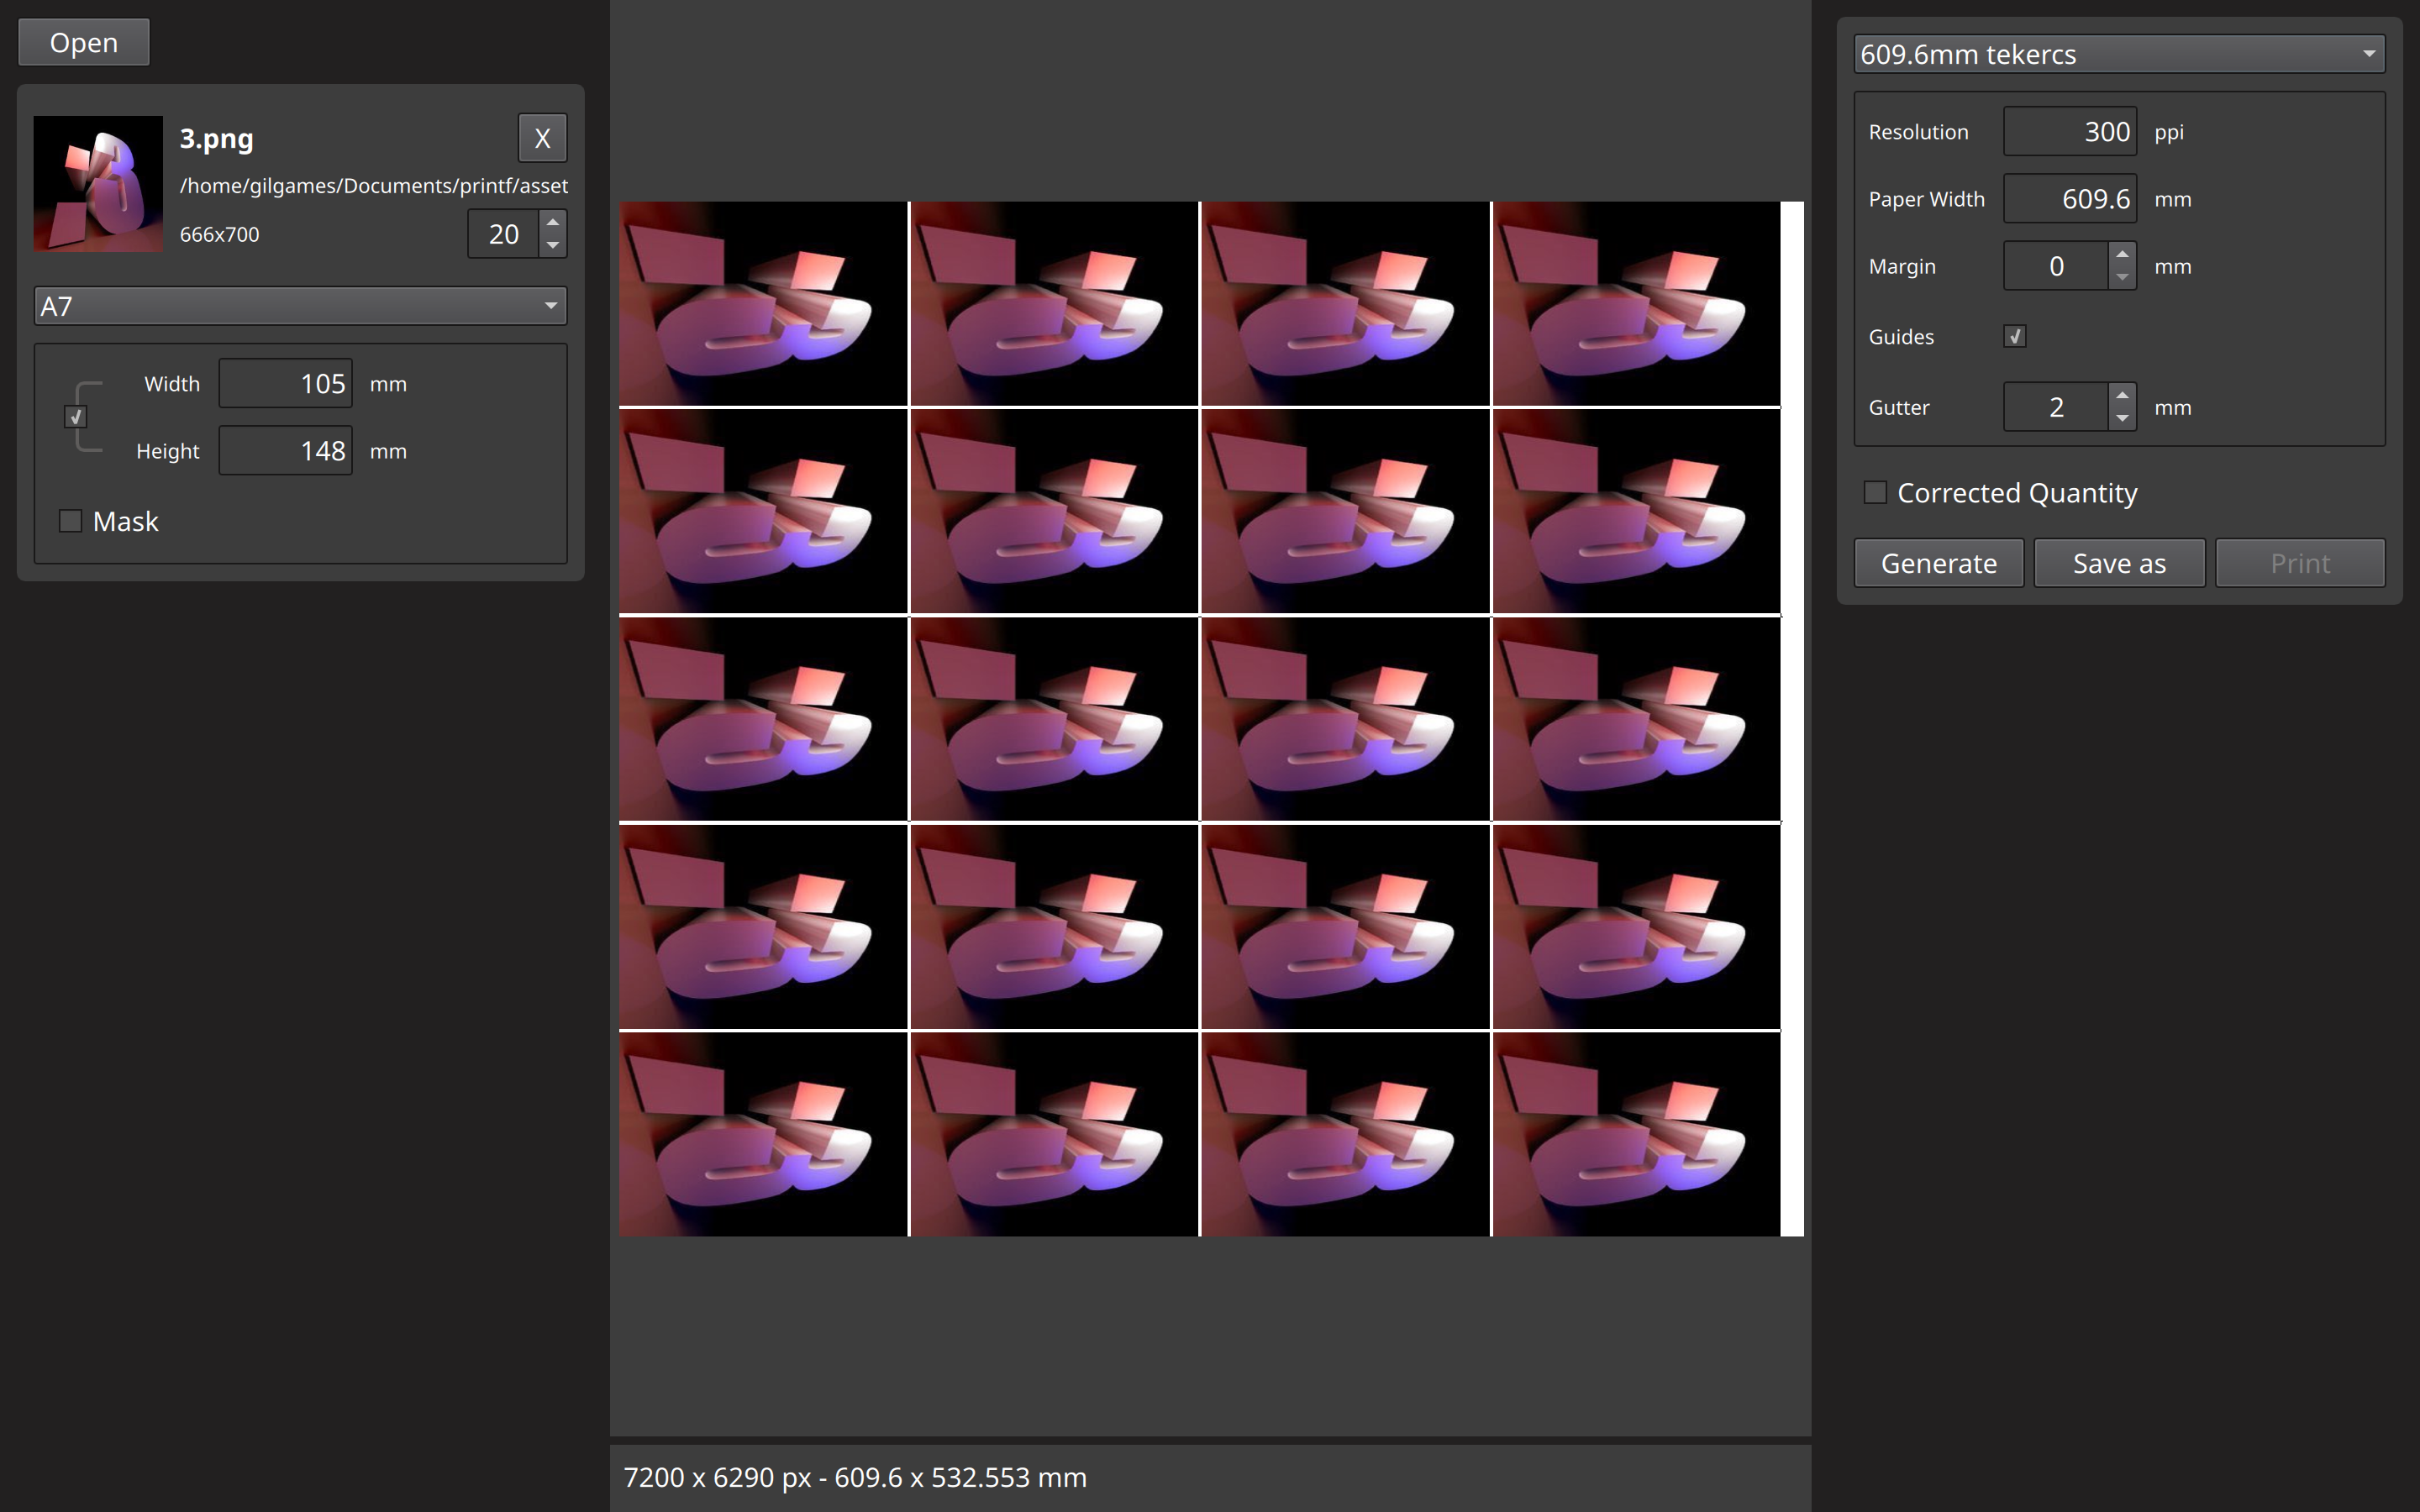
\includegraphics[width=\textwidth]{figures/ui_showcase.png}
    \caption{A felhasználói felület}
    \label{fig:ui_screenshot}
\end{figure}

\subsection{Több szálon futás}

Ugyan ügyeltem, hogy minél gyorsabb legyen a kép generálása, ez a folyamat így is tud időigényes lenni. Itt ugyan csak pár másodpercről beszélünk, de ez elég arra, hogy a Qt felület azt higgye, hogy az alkalmazásunk lefagyott. Ez egy elég gyakori eset a szoftverfejlesztésben, már jól ismert megoldással: tegyük át, hogy ne a fő szálon fusson a generálás. Az implementáció itt sem volt zökkenőmentes, hiszen valahogy jeleznünk is kell a UI felé, hogy frissült az eredmény, de vannak erre ún. signalok. Hasonló problémába ütköztem a kép elmentésénél, ami mégtovább tart, de ezt is ugyan úgy javítani tudtam. 

\subsection{Exportálás}

Miután már a többszálúságot megoldottam a kép elmentése nem kimondottan volt kihívás, mert volt rá beépített függvény. Teszteléskor viszont sajnos kibukott, hogy a nyomtatáshoz használt szoftverünk miatt szükség lenne bizonyos metaadatokra, elsősorban a képpontsűrűségre (dpi), erre viszont a beépített megoldások nem voltak képesek. Először \href{https://en.wikipedia.org/wiki/Exif}{EXIF} metaadatokkal próbáltam megoldani, amit a legtöbb képnézegető meg is jelenít. Windowson viszont kicsit más a helyzet, az ottani file tulajdonságoknál és így a nyomtató szoftverében sem jelent meg beállított dpi. Megpróbáltam valami hasonlót \href{https://en.wikipedia.org/wiki/Extensible_Metadata_Platform}{XMP}-mal is, de hiába. Az egyetlen lehetőségem ami maradt, az az hogy a fájl formátum fejlécben tároljam el. Ez persze formátumonként eltér és más-más implementációk tartoznak hozzá, nem úgy, mint az EXIF-nál. A veszteségmentességéből adódóan a PNG formátum melett döntöttem. Bármennyire is élveztem elmerülni a képformátumok kodekjeinek működésében, nem hiszem hogy ennek a projektnek a kereteiben szeretnék saját PNG tömörítőt írni (nem is beszélve arról, hogy a megoldásom messze nem lenne optimális), ezért különböző könyvtárakkal próbáltam megoldani. A végső megoldás a \href{https://libspng.org/}{libspng} C könyvtárat használja. Igyekeztem elkerülni, hogy másolat készüljön a képről a lemezen vagy a memóriában, ezt sajnos nem egészen sikerült megoldani. 

\subsection{Refaktorálás}

A félév vége felé haladva elkezdtem refaktorálni a forráskódot. Elkezdtem használni a shared és unique pointereket, megelőzve ezzel a legvalószínűbb memóriaszivárgásokat. A kód nincs dokumentálva, de követi a clean code elveit. 
